% Vorlage für eine Bachelorarbeit - 2012-2013 Timo Bingmann

% Dies ist nur eine Vorlage. Strikte Vorgaben wie die Bachelorarbeit auszusehen
% hat gibt es nicht. Darum können auch alle Teile angepasst werden.

\documentclass[12pt,a4paper,twoside]{scrartcl}

% Diese (und weitere) Eingabedateien sind in UTF-8
\usepackage[utf8]{inputenc}

% Verwende gute Type 1 Font: Latin Modern
\usepackage[T1]{fontenc}
\usepackage{lmodern}

% Sprache des Dokuments (für Silbentrennung und mehr)
\usepackage[english]{babel}

% Seitengröße - verwende fast die ganze A4 Seite
\usepackage[tmargin=22mm,bmargin=22mm,lmargin=20mm,rmargin=20mm]{geometry}

% Einrückung und Abstand zwischen Paragraphen
\setlength\parskip{\smallskipamount}
\setlength\parindent{0pt}

% Einige Standard-Mathematik Pakete
\usepackage{latexsym,amsmath,amssymb,mathtools,textcomp}

% Unterstützung für Sätze und Definitionen
\usepackage{amsthm}

\newtheorem{Satz}{Satz}[section]
\newtheorem{Definition}[Satz]{Definition}
\newtheorem{Lemma}[Satz]{Lemma}

\numberwithin{equation}{section}

% Deutsches Literaturverzeichnis
% \usepackage{bibgerm}

% Unterstützung zum Einbinden von Graphiken
\usepackage{graphicx}

% Pakete die tabular und array verbessern
\usepackage{array,multirow}

% Kleiner enumerate und itemize Umgebungen
\usepackage{enumitem}

\setlist[enumerate]{topsep=0pt}
\setlist[itemize]{topsep=0pt}
\setlist[description]{font=\normalfont,topsep=0pt}

\setlist[enumerate,1]{label=(\roman*)}

% TikZ für Graphiken in LaTeX
\usepackage{tikz}
\usetikzlibrary{calc}
\usepackage{subcaption}
\usepackage{booktabs}

% Aktuelle Section und Untersection am Seitenkopf
\usepackage{fancyhdr}

\fancypagestyle{plain}{
  \fancyhead{}
  \fancyfoot{}
  \fancyfoot[LE,RO]{\normalsize\thepage}
  \renewcommand{\headrulewidth}{0pt}
  \renewcommand{\footrulewidth}{0pt}
}

\fancypagestyle{normal}{
  \setlength{\headheight}{20pt}
  \setlength\footskip{32pt}
  \fancyhead{}
  \fancyhead[LE]{\normalsize\textsc{\nouppercase{\leftmark}}}
  \fancyhead[RO]{\normalsize\textsc{\nouppercase{\rightmark}}}
  \fancyfoot{}
  \fancyfoot[LE,RO]{\normalsize\thepage}
  \renewcommand{\headrulewidth}{0.4pt}
  \renewcommand{\footrulewidth}{0pt}
}

% Hyperref für Hyperlink und Sprungtexte
\usepackage{xcolor,hyperref}

\hypersetup{
  pdftitle={Combining Memory-Efficient Parallel SAT Solving and Distributed Clause Sharing},
  pdfauthor={Ruben Götz},
  pdfsubject={},  % TODO: add tags
  colorlinks=true,
  pdfborder={0 0 0},
  bookmarksopen=true,
  bookmarksopenlevel=1,
  bookmarksnumbered=true,
  linkcolor=blue!60!black,
  %linkcolor=black,
  citecolor=blue!60!black,
  urlcolor=blue!60!black,
  filecolor=green!60!black,
  pdfpagemode=UseNone,
  unicode=true,
}

% Paket zum Setzen von Algorithmen in Pseudocode mit kleinen Stilanpassungen
\usepackage[ruled,vlined,linesnumbered,norelsize]{algorithm2e}
\DontPrintSemicolon
\def\NlSty#1{\textnormal{\fontsize{8}{10}\selectfont{}#1}}
\SetKwSty{texttt}
\SetCommentSty{emph}
%\def\listalgorithmcfname{Algorithmenverzeichnis}
\def\algorithmautorefname{Algorithmus}
\let\chapter=\section % repariert ein Problem mit algorithm2e

\usepackage{longtable}

\begin{document}

%%%%%%%%%%%%%%%%%%%%%%%%%%%%%%%%%%%%%%%%%%%%%%%%%%%%%%%%%%%%%%%%%%%%%%

\pagestyle{empty} % keine Seitenzahlen

% Titelblatt der Arbeit
\begin{titlepage}

  \begin{center}\large

    \quad\includegraphics[height=17mm]{kit_logo_de.pdf} \hfill
    \includegraphics[height=20mm]{grouplogo-algo-blue.pdf}\quad\null

    \vfill

    Master Thesis
    \vspace*{2cm}

    {\huge 	Combining Memory-Efficient Parallel SAT Solving and Distributed Clause Sharing \par}
    % Siehe auch oben die Felder pdftitle={}
    % mit \par am Ende stimmt der Zeilenabstand

    \vfill

    Ruben Götz

    \vspace*{15mm}

    15. August 2025

    \vspace*{45mm}

    \begin{tabular}{rl}
      Betreuer: & Prof. Dr. Peter Sanders \\
      & Dr. rer. nat. Dominik Schreiber \\
    \end{tabular}
    
    \vspace*{10mm}

    % Institut für Theoretische Informatik, Algorithmik \\
    % Fakultät für Informatik \\
    % Karlsruher Institut für Technologie

    % English:
    Institute of Theoretical Informatics, Algorithmics \\
    Department of Informatics \\
    Karlsruhe Institute of Technology

    \vspace*{12mm}
  \end{center}

\end{titlepage}

%%%%%%%%%%%%%%%%%%%%%%%%%%%%%%%%%%%%%%%%%%%%%%%%%%%%%%%%%%%%%%%%%%%%%%

\vspace*{0pt}\vfill

\hrule\medskip

Hiermit versichere ich, dass ich diese Arbeit selbständig verfasst und keine anderen, als die angegebenen Quellen und Hilfsmittel benutzt, die wörtlich oder inhaltlich übernommenen Stellen als solche kenntlich gemacht und die Satzung des Karlsruher Instituts für Technologie zur Sicherung guter wissenschaftlicher Praxis in der jeweils gültigen Fassung beachtet habe.

\bigskip

\noindent
Ort, Datum

% Unterschrift (handgeschrieben)

\vspace*{5cm}

\clearpage

%%%%%%%%%%%%%%%%%%%%%%%%%%%%%%%%%%%%%%%%%%%%%%%%%%%%%%%%%%%%%%%%%%%%%%

\vspace*{0pt}\vfill

% \selectlanguage{english}
% \begin{abstract}
% \centerline{ Zusammenfassung}
%
% Hier die deutsche Zusammenfassung
%
% \end{abstract}
%
% \vfill

\selectlanguage{english}
\begin{abstract}
\centerline{Abstract}
  TODO: write some Abstract.
\end{abstract}
\selectlanguage{english}

\vfill\vfill\vfill
\clearpage

%%%%%%%%%%%%%%%%%%%%%%%%%%%%%%%%%%%%%%%%%%%%%%%%%%%%%%%%%%%%%%%%%%%%%%

% \vspace*{0pt}\vfill
% 
% \section*{Danksagungen}
% 
% 
% \vfill\vfill\vfill
% \clearpage

%%%%%%%%%%%%%%%%%%%%%%%%%%%%%%%%%%%%%%%%%%%%%%%%%%%%%%%%%%%%%%%%%%%%%%

\pagestyle{normal}
% markiere sections im Seitenkopf links und subsections rechts
\renewcommand\sectionmark[1]{\markboth{\thesection\quad\MakeUppercase{#1}}{\thesection\quad\MakeUppercase{#1}}}
\renewcommand\subsectionmark[1]{\markright{\thesubsection\quad\MakeUppercase{#1}}}

% Inhaltsverzeichnis
\tableofcontents

\clearpage

%%%%%%%%%%%%%%%%%%%%%%%%%%%%%%%%%%%%%%%%%%%%%%%%%%%%%%%%%%%%%%%%%%%%%%

\listoffigures
\listoftables
% \listofalgorithms

\clearpage

%%%%%%%%%%%%%%%%%%%%%%%%%%%%%%%%%%%%%%%%%%%%%%%%%%%%%%%%%%%%%%%%%%%%%%

\section{Introduction}

TODO: write some introduction into parallel sat solving in general

\subsection{Motivation}

Memory in Cloud applications can be expensive or highly limited on slim processing nodes. We thus want to try to limit memory consumption by combining gimsatul -- a shared memory clause sharing satsolver -- with the hyper parallel sat-solver MallobSat.\\

TODO: make motivation a meaningfull paragraph

\subsection{Contribution}

Combined two clause sharing approaches.\\

TODO: an overview over what we did in this thesis


%%%%%%%%%%%%%%%%%%%%%%%%%%%%%%%%%%%%%%%%%%%%%%%%%%%%%%%%%%%%%%%%%%%%%%

\section{Preliminaries And Related Work}

\subsection{Definitions}

TODO: some Definitions used in this thesis. Probably a fairly small section due to the emphasis on engineering.

\begin{itemize}
  \item glue and lbd values
\end{itemize}

\subsection{Related Work}

TODO: talk about sat solving in general

\subsubsection{Parallel SAT-Solving}

TODO: talk about the state of the Art in parallel SAT-Solving

\subsubsection{Memory Efficient SAT-Solving}

TODO: talk about approaches that have been taken to reduce memory demand in parallel sat-solving.

%%%%%%%%%%%%%%%%%%%%%%%%%%%%%%%%%%%%%%%%%%%%%%%%%%%%%%%%%%%%%%%%%%%%%%

\section{The Algorithm}

In this section we want to introduce MallobSat and Gimsatul, the core building blocks of our work. We integrated Gimsatul into MallobSat as a Solver backend to utilize both Gimsatul's memory efficiency, achieved by shared memory clause sharing, and MallobSat's massively parallel scalability. We also want to describe the architecture we used to make it possible to use the already parallel SAT-solver Gimsatul as a solver backend in MallobSat.

\subsection{MallobSat}

MallobSat \cite{mallobSat} is a massively parallel SAT-solver that categorizes itself as a clause-sharing solver rather than the more common term 'portfolio solver', due to its focus on clause sharing and paradigm of treating solver engines as blackbox serial SAT-solvers. In this section we want to give a broad overview over MallobSat's architechture and only describe the systems that we had to adapt in more detail. A complete record of MallobSat's inner workings can be found in its dedicated paper by Schreiber et al. \cite{mallobSat}.

On an abstract view MallobSat combines existing serial SAT-solvers into a massively parallel distributed and malleable SAT-solver system by implementing a Clause sharing interface and the necessary infrastructure to manage and exchange derived clauses between these so called solver engines. It accomplishes this by grouping solver engines into processes and creating a clause sharing system for these processes on top.

TODO: adapt Mallob Engine graphic

MallobSat equips each process with a fixed size import buffer for each of the processes solver engines and a single fixed size export buffer that is shared between all solver engines in a process. The processes are organized into a distributed binary tree to enable clause sharing for distributed systems. The exchange of clauses between processes happens periodically. In the world of MallobSat the times between these so called 'collective sharing operations' are called epochs.
%An epoch $e \geq 0$ starts with the sharing operation $e$, i.e. the first epoch $e = 0$ starts with the beginning of solving, the second epoch $e = 1$ beginns with the first sharing operation and so on.
At the beginning of each epoch (besides the first one) a collective sharing operation is executed: Each process is combining its own export buffer with the ones of its children, filtering duplicate clauses along the way. This process is executed from the leafs up to the root of the binary communication tree. If the merged export buffer exeeds its limit, clauses are discarded by their priority. MallobSat prioritizes clauses first by length, then by their lbd value and finally lexicographically as a tie breaker. If the root process has recieved the merged export buffers, the resulting collection of clauses is then broadcast down the binary tree.

Clause sharing from the perspective of a solver engine inside a process happens asynchonously: If a solver engine has deduced a clause it sees fit to be shared, the engine simply writes this clause into an export buffer and executes a callback method provided by MallobSat at any time. If a a solver engine is ready to import external clauses (usually when restarting) it can iterate through its dedicated import buffer and import clauses from there. Usually an engine then has to do some filtering of its own, e.g. not to import clauses it already derived itself or clauses containing literals the engine already marked as inactive. Engines might also want to shorten clauses even more, if it already falsified some literals contained in the newly imported clause.

To keep the communication volume as low as possible and to make sure important clauses are not lost to overflowing buffers, MallobSat employs some highly soffisticated filtering mechnanisms for clauses that are im- and exported by solver engines. We treat these filter mechanism as blackboxes going forward. Like we mentiond earlier in this section, the interested reader is referred to the detailed description by Schreiber et al. in their dedicated paper \cite{mallobSat}.

\subsection{Gimsatul}

Gimsatul \cite{gimsatul} is a paralell portfolio SAT-solver that aims to reduce its memory consumption and enable agressive clause sharing by using a shared memory approach for its clauses. The solver engines are CDCL solvers. In the world of Gimsatul these solver threads are called rings. There also exists a ruler thread, handeling initialisation and synchonisation of its rings. We will adopt this naming pattern from here on out when talking about Gimsatul's inner workings.

Gimsatul achieves its shared memory approach for clauses by only sharing pointers to newly derived clauses instead of whole clause themselfs. To make this possible Fleury and Biere revisit the classical watcher data structures, resulting in all rings sharing their clauses in memory but maintaining their own watcher data structures independently. Further details are given in the original paper \cite{gimsatul}.

We do want to recap Gimsatul's clausesharing mechnanisms more closely however, since this will become importatnt later on. If a ring derives a clause it deems worthy to share (i.e. a clause with a low glucose level) it will store a reference to this clause inside a buffer of small constant size for each other ring. If a buffer is full it will throw out the clause with the highest glucose level in the buffer. When a ring decides to import a clause it will pick another ring at random and import the clause with the lowest glucose level in it's respective buffer.

TODO: adapt Gimsatul's clause sharing graphic

To diversify the rings Gimsatul utilizes differing initialisations for the first random walks of each ring. Each ring can start this procedure with either all phases set to 1 or all phases set to 0. Again more detail is given in the original paper \cite{gimsatul}.

\subsection{Architecture}

We now want to describe the architectue of our algorithm, integrating Gimsatul (and with it its memory efficient shared memory approach) as a solver engine into MallobSat. In the following we will use 'external' and 'internal' when talking about our architecture w.r.t. MallobSat from the point of few of a Gimsatul instance. E.g. When rings of a Gimsatul instance exchange derived clauses we will denote this as 'internal clause exchange', if a Gimsatul instance is exchanging clauses as a solver engine in MallobSat we will call this 'external clause exchange'.

The most intuitive approach to integrate Gimsatul into MallobSat would be to consider each ring in a Gimsatul instance as a solver engine in MallobSat, complying with MallobSat's paradigm of each solver engine beeing an independent serial SAT-solver. This approach runs into some fundamental problems however: 
First off, Gimsatul is initialized by reading the original CNF Formula of a given Problem, running some preprocessing, initializing a single ring and then cloning said ring $t - 1$ times to create its $t$ solving threads (i.e. rings). If we integrated each ring to be a solver engine in MallobSat we would have to reimplement all of Gimsatul's initialisation to create each ring independently. This would make it unfeasible to keep Gimsatul's shared memory Clauses.
Even more problematic would be MallobSat's malleability though. MallobSat is able to handle a fluctuating number of solver engines. If necessary it will make use of its malleability and stop / restart some of them. Gimsatul does not share this malleability. We thus would have to redesign its thread management.

For the above mentioned reasons we decided to implement a (in our opinion) more elegant architechture, shown in figure \ref{fig:architecture}: We adapted Gimsatul to be a single solver engine in MallobSat, thus avoiding the initialisation and malleability problems with Gimsatul.

\begin{figure}
  \center
  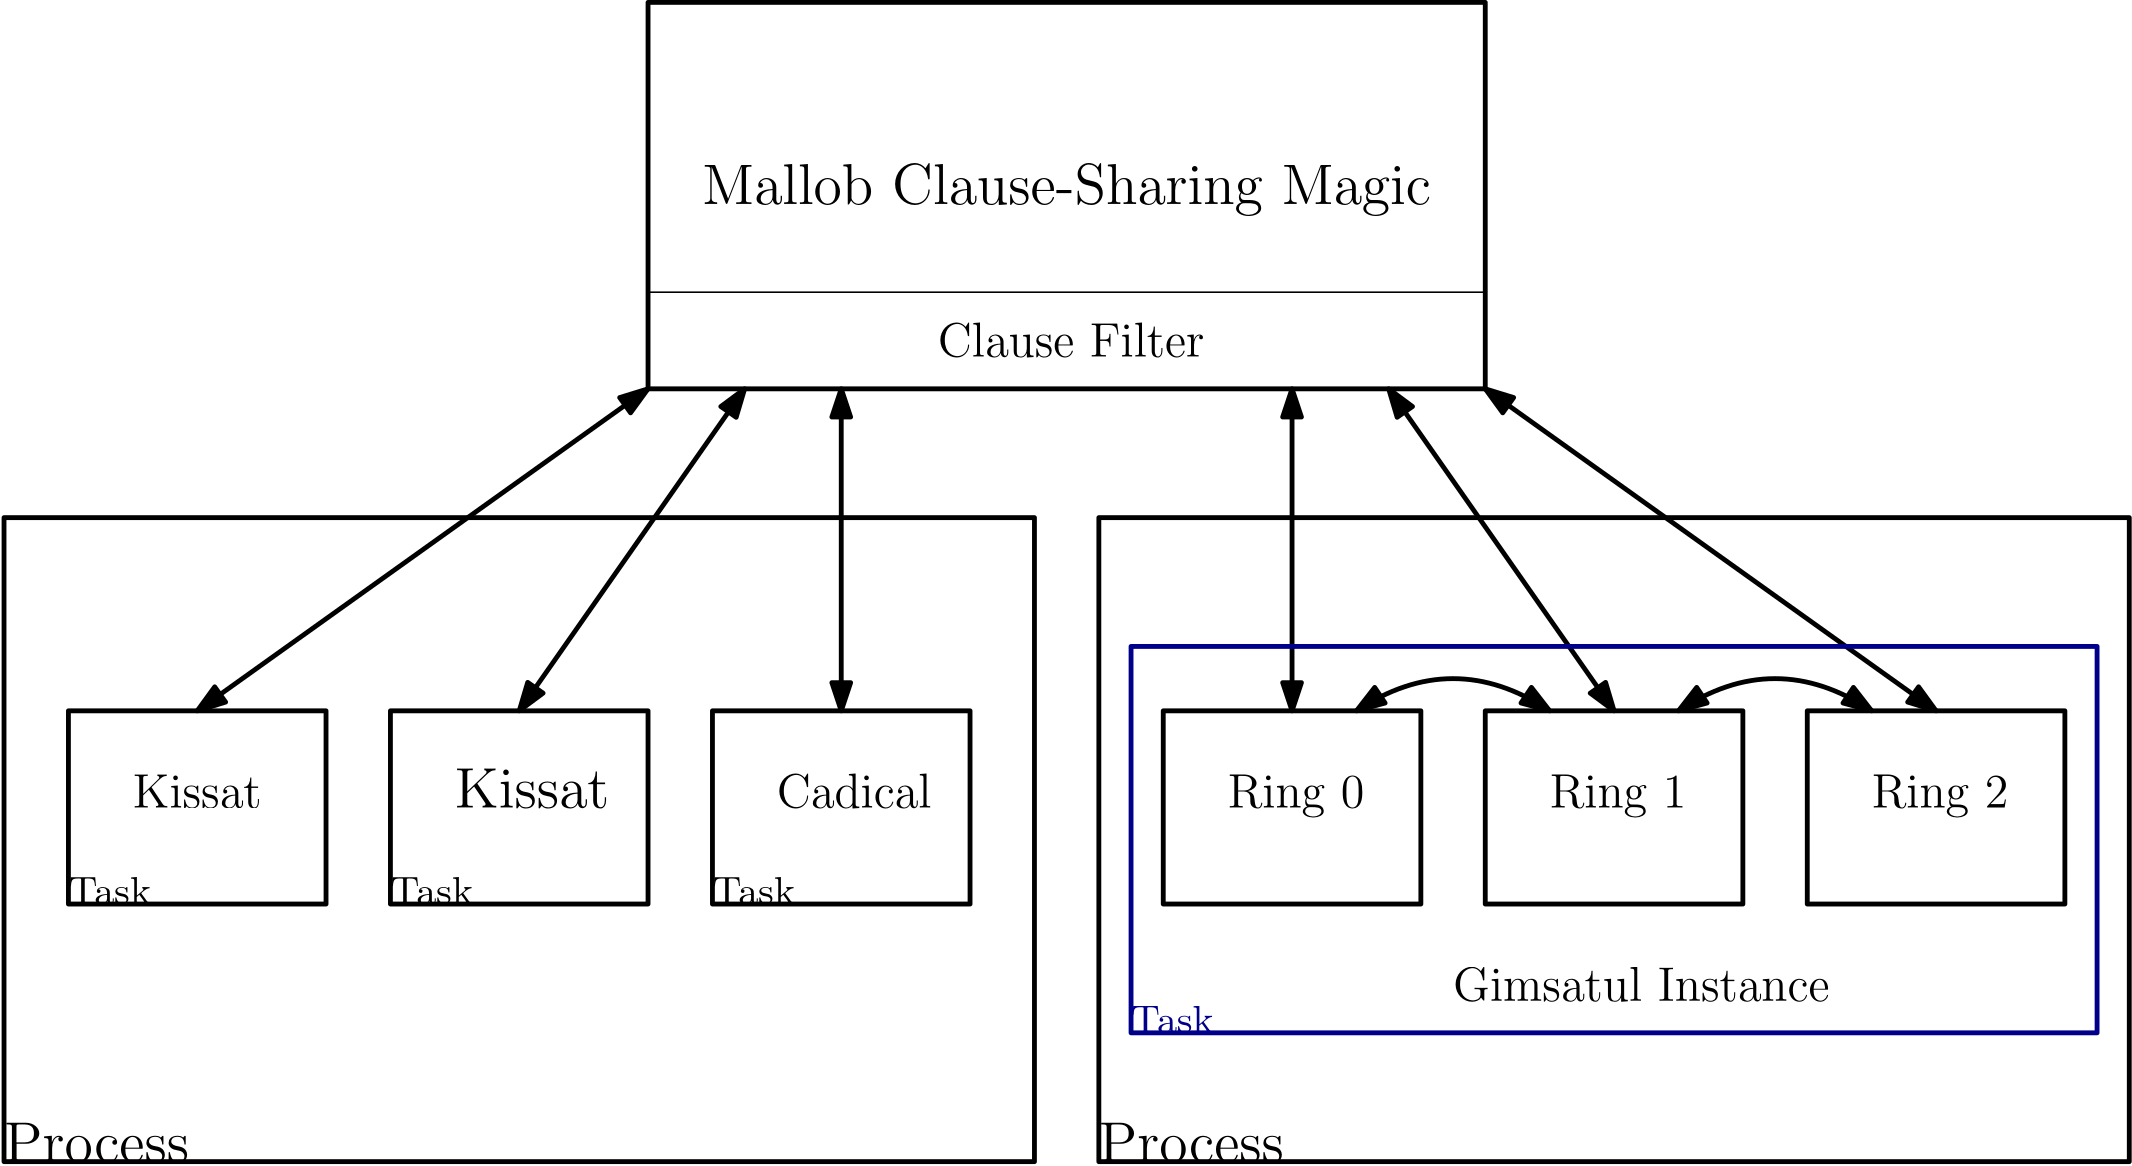
\includegraphics[scale=.2]{figures/architektur.png}
  \caption{Architecture. TODO: make pretty}
  \label{fig:architecture}
\end{figure}

\subsubsection{Creating the Solver Engine}

MallobSat assumes its solver engines to be serial blackbox sat solvers leaving us with the challange to fiddle with MallobSat's engine setup, so that our multi threaded Gimsatul Instance looks and behaves like a serial SAT-solver.
When initializing a process with $t$ solver engines, i.e. threads, MallobSat creates a portfolio of $t$ solvers from a given regular expression that defines the portfolio for the execution of MallobSat. We adapted this procedure to akkumulate all $t' \leq t$ threads that are defined to be Gimsatul threads into a single solver engine and then run Gimsatul with $t'$ threads. The MallobSat process now contains $t - t'$ solver engines and operates like the process runs with $t - t'$ threads -- at most one of them beeing a Gimsatul Instance.

MallobSat and Gimsatul both implement some diversification over their respective threads (i.e. solver engines / rings). Since Gimsatul runs multiple rings inside a single solver engine we also had to adapt both these procedures to wirk in tandem.
The biggest part of MallobSat's diversification that actually has to be supported by the solver engine and is not done on a meta level over multiple engines are the so called 'sparse random variable phases', originally introduced by Balyo et al. \cite{hordeSat}. This procedure flips the phases of random literals in a solver engine with probability $1 / e$ for a run with $e$ engines in total. Each process runs this algorithm with $e = t * p$, where $t$ denotes the number of engines in a process and $p$ denotes the number of processes. Since Gimsatul runs with multiple threads we can not na\"ively flip its phases like we could with a serial solver engine. Instead of flipping the phases given by MallobSat our Gimsatul engine calculates and applies the sparse random variable phases for its $t'$ rings itself (i.e. flipping a phase with probability $1 / (t' * p)$). If a process runs with a single Gimsatul engine this results in the same outcome.
Gimsatul's native diversification only ever applies the same phase for all its variables. We added the calculated sparse random variable phases on top of Gimsatul's diversification by flipping the respective initial phases of a ring.

\subsubsection{Clause Export}

To export clauses from Gimsatul we took the simplest possible approach by latching the MallobSat clause export to Gimsatul's native internal clause export\footnote{Since Gimsatul does not trigger its clause sharing routines when executed with a single thread, it will also only export its derived clauses to MallobSat when run with at least 2 threads. Since our focus is on memory efficiency we do not see any reasons to run Gimsatul with a single thread and therefore do not consider this a problem.}. The reasoning beeing that if Gimsatul consideres a clause to be good enough to be shared internally it is good enough to be shared externlly through MallobSat. This might not always be the case however, since Gimsatul is sharing clauses fairly aggressively -- capitalizing on its shared memory approach to not have to copy the shared clauses on each export. Rather than implementing additional heuristics to differentiate between clauses that should be exported to other rings only and clauses that should be shared globally through MallobSat we decided to rely on MallobSat's sophisticated clause filtering. Thus incidentally saving on the additional execution time a complementary heuristic would entail.

Since MallobSat sees Gimsatul as a single solver engine it naturally keeps track of all the rings' clauses as beeing produced by a single thread, preventing redundant clause sharing through Gimsatul and MallobSat.

\subsubsection{Clause Import}

Usually MallobSat's solver engines import all the external clauses stored in their import buffer every time they do a restart. This way they are importing on decision level zero and do not have to consider their current state when deciding whether to keep the imported clauses. 

Importing external clauses into Gimsatul turned out to be a bit more complex though. Since we integrated Gimsatul as a single solver engine into MallobSat, we had to work with a single import buffer. MallobSat's import buffers are built in a way that clauses are immediatly deleted when read by the solver engine. We want to reason our approach by first discussing two scrapped approaches.

\textbf{Rings import independently.} To make it possible for every ring to read the import buffer independently we would have had to redesign both MallobSat's import buffers, and Gimsatul's clause lifecycle. The import buffers would need some functionality to keep track of which rings had already read which clauses. And Gimsatul' rings would have needed some functionality to import only the reference to a clause, if it had already been imported into the shared memory by another ring. 

\textbf{Single dedicated importing ring.} Having a dedicated ring to import all clauses from the import buffen whenever it does a restart left the challange of spreading the imported external clauses through all of Gimsatul's rings. This approach already resulted in some scalability improvements over vanilla Gimsatul. However, since Gimsatul's internal clause sharing utilizes buffers of extremely limited size, importing the full import buffer from MallobSat all at once and immediatly exporting them internally in Gimsatul would dicard many of the external clauses by overflowing internal buffers.

\textbf{Our approach.} We combined the afore mentioned approaches to spread externally imported clauses throughout Gimsatul's rings without having to import an external clause multiple times by letting each ring exclusively import a small set of clauses from MallobSat's import buffer: 
In our approach all rings try to import clauses from MallobSat's import buffer when restarting. To avoid race conditions and to minimize active waiting times we allow only one ring to import external clauses at a time. We utilize an atomic flag to indicate wether a ring is currently importing external clauses. If a ring is restarting and the flag is not set (i.e. no other ring is currently importing) it starts it's the importing routine. If the flag is set (i.e. some other ring is currently importing) it continues its solving routine to avoid actively waiting. 
When a ring is importing external clauses they are handled like they were deduced by the importing ring and instantly internally exported to eventually spread them throughout all rings. 
% Annahme: das funktioniert. Ich kann zur Zeit nicht auf superMUC zugreifen :(
To avoid overflowing Gimsatul's internal export buffers, a ring checks all of said export buffers for free slots before importing. It then only imports at most so many external clauses, that no overflows occour. For example: If we run a Gimsatul instance with 3 rings as a solver engine in MallobSat and ring 0 tries to import some external clauses it will check its export buffers for ring 1 and 2 and might find them to have 4 and 6 free slots respectively. It will then import at most 4 clauses from MallobSat's import buffer.

%%%%%%%%%%%%%%%%%%%%%%%%%%%%%%%%%%%%%%%%%%%%%%%%%%%%%%%%%%%%%%%%%%%%%%

\newpage
\section{Experimental Evaluation}

In this section we want to discuss the findings of our experimental results of our algorithm. All experiments in this section were conducted on the superMUC-NG cluster equiped with Intel Skylake Xeon Platinum 8174 processors. We evaluated our Algorithm on up to 16 of the the superMUC-NG's thin nodes, all containing 48 cores (96 hardware threads) with 96GB memory.

TODO: SuperMUC citation? I didnt find anything...

\subsection{Benchmarks}
To evaluate our algorithm we used benchmark instances provided by Iser et al. on their Global Benchmark Database \cite{benchmarkDB}. Specifically we used the 400 instances contained in the track main\_2024 that was used in the 2024 SAT competition \cite{satComp2024}, containing a myriad of different problems encoded as SAT instances.

\subsection{Configuration}
We ran our Algorithm with one gimsatul instance per node, i.e. 48 threads in one shared memory instance. Running multiple Gimsatul instances on the same node proved to yield comparable or worse results to only one instance per node with significant memory costs. Using the nodes capability of hyperthreading to exploit all 96 virtual threads was not supported by Mallob on the superMUC-NG cluster. We would not expected an increase in performance in this case regardles, since in all cases the configurations utilizing hall 96 virtual nodes performed worse that their counter parts with only the 48 hardware threads. Figure \ref{fig:1nodeConfigCompare} shows our results for all the thread configurations we tested on one node. To save on computing time, we reason that the best configuration for one node will also be the best for multiple nodes instead of testing them all on multiple nodes. To reinforce this argument we tried the best two configurations for one node on 2 compute nodes as shown in figure \ref{fig:2nodeConfigCompare}. In the following we will denote the two configurations as follows:
\begin{itemize}
  \item[$A$:] 1 Gimsatul instance with 48 threads per node
  \item[$B$:] 2 Gimsatul instances with 24 threads each per node
\end{itemize}
In our experiments configuartion $B$ solved 10 benchmark instances, that configuration $A$ did not solve within a 300s time limit. Of these 10 instances 7 were SAT and thus some of them may be contributed to lucky non determinism. Configuration $B$ solved 3 instances, that configuration A could not solve within the time limit. We opted for the configuration $A$ mainly for for its significantly more efficient memory usage as shown in figure \ref{fig:2nodeConfigMemCompare}.

\begin{figure}
  \center
  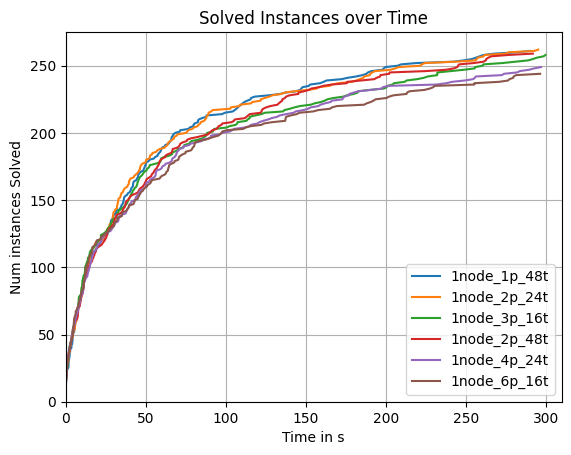
\includegraphics{plots/config_compare/1node_config_compare.png}
  \caption{Comparison between thread configurations on a single node.}
  \label{fig:1nodeConfigCompare}
\end{figure}

\begin{figure}
  \center
  \begin{subfigure}[c]{0.4\textwidth}
    \center
    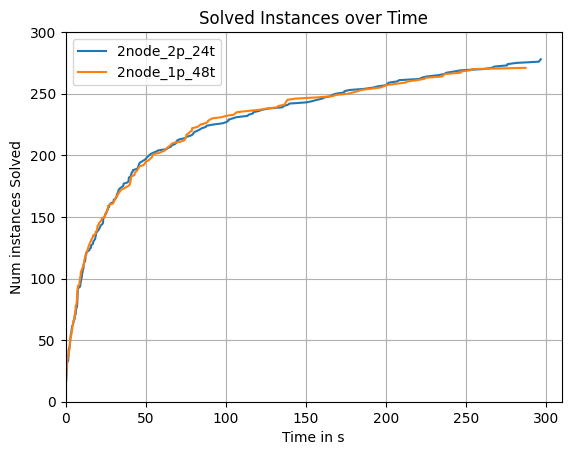
\includegraphics[scale=0.5]{plots/config_compare/2node_config_compare.png}
    \caption{}
    \label{2nodeConfigRuntimeCompare}
  \end{subfigure}
  \hfill
  \begin{subfigure}[c]{0.4\textwidth}
    \center
    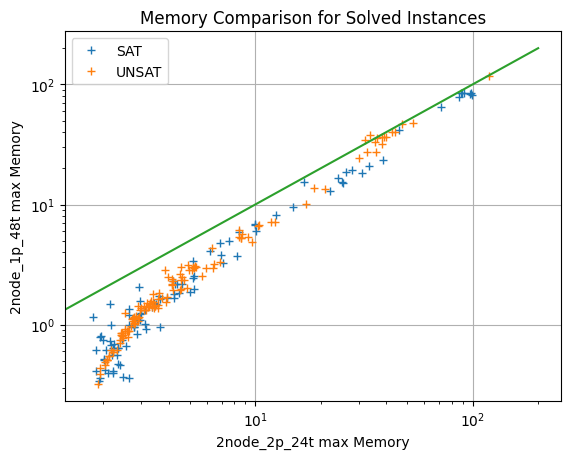
\includegraphics[scale=0.5]{plots/config_compare/2node_config_mem_compare.png}
    \caption{}
    \label{fig:2nodeConfigMemCompare}
  \end{subfigure}
  \caption{Comparison between thread configurations on two nodes.}
  \label{fig:2nodeConfigCompare}
\end{figure}

To further configure MallobSat's options we implemented a search only approach with only a single preprocessor as introduced by Schreiber et al. \cite{searchOnlyPaper}. To do this we deactivated all pre- and inprocessing procedures in our Gimsatul instances, i.e. no simplifying or probing. For Gimsatul this has the additional effect of avoiding the synchronization between all rings of a Gimsatul instance. This increases memory consumption due to missing compacting procedures but avoids idleing rings while waiting for other rings to synchonize. To preprocess the formula we utilized the Kissat SAT-solver \cite{kissat}. We found a significant increase in performance due to this practice. (TODO: give a figure? This experiment was only run on the institute servers...)

\subsection{Runtime and Memory Usage}

We first want to discuss our findings on runtime regarding the scalability on up to 16 nodes (i.e. 768 processors). We then compare our Algorithm to the state of the art distributed SAT-solver MallobSat with its default configuration utilizing one Kissat instance per processor.

\subsubsection{Speedups}

As shown in figure \ref{fig:runtimeCompareGim} we ran our algorithm on 1, 2, 4, 8 and 16 nodes respectively. We can see an increase in performance with an increasing amount of available processing power, albeit with deminishing returns.

\begin{figure}
  \center
  \begin{subfigure}[c]{\textwidth}
    \center
    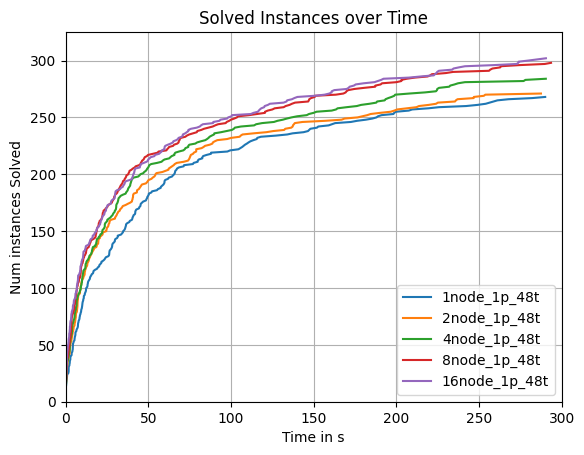
\includegraphics{plots/cumulative_runtime/scalability_gim.png}
    \subcaption{Scalability Our Approach}
    \label{fig:runtimeCompareGim}
  \end{subfigure}
  \hfill
  \begin{subfigure}[c]{\textwidth}
    \center
    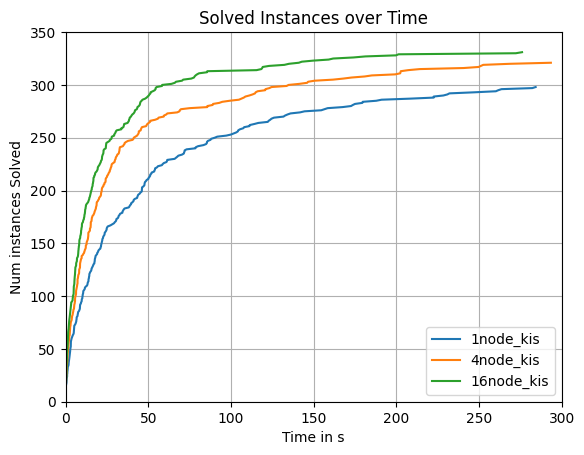
\includegraphics{plots/cumulative_runtime/scalability_kis.png}
    \subcaption{Scalability MallobSat}
    \label{fig:runtimeCompareKis}
  \end{subfigure}
  \caption{Some Example plot on scalability}
  \label{fig:scale}
\end{figure}

To calculate Speedups we ran the sate of the art serial SAT-solver Kissat for up to 3000s on a single processor. The results of this run are shown in figure \ref{fig:runtimeSerial}. The geometric means over all speedups for benchmark instances solved by Kissat are shown in table \ref{tab:speedups}. We can see an increase in the geometric mean speedup for our algorithm with increasing amounts of processors, albeit with deminishing returns. The specific speedups for all instances that were solved by Kissat in a timelimit of 3000s are shown in figure \ref{fig:speedups}. Here we can observe a great variance in speedups for simple instances (i.e. instances Kissat solved in under 500 seconds). For complex instances (i.e. instances where Kissat needed more than 500 seconds) we can see a tendency for the speedups to become greater. For really complex instances the speedups routily beat the geometric mean while their variance increases even more.

\begin{figure}
  \center
  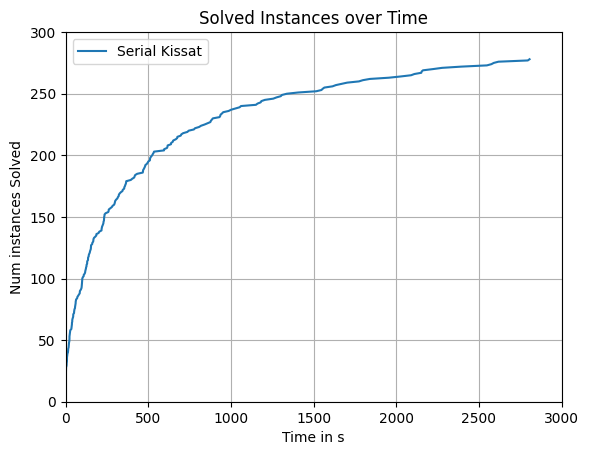
\includegraphics{plots/cumulative_runtime/runtime_serial.png}
  \caption{Scalability of serial Kissat}
  \label{fig:runtimeSerial}
\end{figure}

\begin{table}
  \center
  \begin{tabular}{ cccc }
    \toprule
    \multicolumn{2}{c}{Setup} & \multicolumn{2}{c}{Solver}\\
    \#nodes   & \#processors   & Our Algorithm  & MallobSat \\
    \midrule
    1  & 48  & 5.389  & 7.847\\
    2  & 96  & 7.376   & -\\
    4  & 192 & 8.027   & 14.034\\
    8  & 384 & 9.425    & -\\
    16 & 762 & 10.185   & 20.073\\
    \bottomrule
  \end{tabular}
  \caption{Geometric mean speedups for number of processors}
  \label{tab:speedups}
\end{table}

\begin{figure}
  \center
  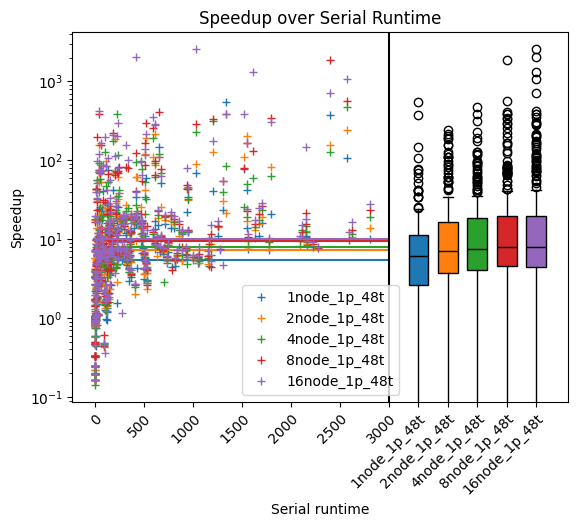
\includegraphics{plots/speedups_gim.png}
  \caption{Speedups of our Algorithm. TODO: make plot pretty}
  \label{fig:speedups}
\end{figure}

%%
% Speedup < 1:
%   cryptography-simon: 10/10   alle sat
%   heule-folkman: 3/11   alle sat
%   maxsat-optimum: 1/13
%   miter: 9/47
%   planning: 1/6 alle unsat
%   reg-n: 2/4 alle unsat
%   scheduling: 2/50
%   software-verification: 2/15 alle unsat
%   subgraph-isomorphism: 2/4   die beiden sat sind langsamer, die beiden unsat schneller

Table \ref{tab:speedupsSignificantFamilies} shows speedups seperated by significant families. By this we mean families with at least 5 Instances contained in our benchmark set. A complete table over all instance families is given in the appendix \ref{app:speedupsFamiliesComplete}. We calculated the geometric mean speedups per family for all our configurations and ordered them by the geometric mean speedup over all 5 configurations.

TODO: is "negative speedup" correct?

For all instances of the family 'cryptography-simon' we found a negative speedup for all setups of our algorithm, which may suggest a systematic discompatibility between our approach and this kind of problem. All Instances of the family 'cryptography-simon' in our benchmark set however were solved in under $0.01s$ by Kissat. Since the fastest meassured runtime of our approach is $0.030417s$ for the instance 'simon-r24-1.sanitized' we attribute any slowdown for instances below $0.03s$ to our increased startup overhead in relation to Kissats serial startup.

For instances of the family 'heule-folkman', which encode proofs whether a graph is a so called Folkman Graph \cite{satComp2024} we find serial Kissat to perform generally better than our approach. In our experiments Kissat solved all $10$ instances of this family in our benchmark set while our approach only solved at most $3$ as shown in table \ref{tab:heuleFolkman}. We currently can not give a specific reason for this phenomenon, however Schreiber et al. \cite{searchOnlyPaper} also found the search only approach in MallobSat to be non-beneficial on this family of instances. We therefore conclude that some inprocessing techniques applied by Kissat make huge improvements in this case. Since we deactivated all pre- and inprocessing to improve overall performance our approach seems to be unsuitable for the 'heule-folkman' family.

TODO: what's up with rbsat? I cant find any info about the family...

Instances of the family 'minimum-disagreement-parity' \cite{satComp2022} encode the minimum disagreement parity problem, which is of interest to the cryptography community and results in challenging SAT problems. This is underlined by the small size of these instances: The biggest one contains only 1021 Variables, with the one that was solved slowest by Kissat (2617.82s) only containing 750 Variables. The family is comprised of 3 satisfiable and 3 unsatisfiable instances. Our high geometric mean speedups of over 29 suggest, the MDP problem instances profit from the increased processing power of parallel sat solving way more than other kinds of problems.

\begin{table}
  \center
  \begin{tabular}{ cc }
    \toprule
    Solver  & \#Instances solved\\
    \midrule
    Kissat  & 10\\
    1node   & 1\\
    2node   & 1\\
    4node   & 1\\
    8node   & 2\\
    16node  & 3\\
    \bottomrule
  \end{tabular}
  \caption{Number of instances solved out of the 10 instances from the Family 'heule-folkman'.}
  \label{tab:heuleFolkman}
\end{table}

\begin{table}
  \center
  \begin{tabular}{ cccccccc }
    \toprule
    family	&	\#	&	1node	&	2node	&	4node	&	8node	&	16node	&	geometric mean\\
    \midrule
    %coloring	&	8	&	-1.0	&	-1.0	&	-1.0	&	-1.0	&	-1.0	&	-1.0\\
    cryptography-simon	&	10	&	0.219	&	0.202	&	0.201	&	0.292	&	0.228	&	0.226\\
    heule-folkman	&	11	&	0.486	&	0.43	&	0.467	&	0.519	&	0.427	&	0.465\\
    miter	&	47	&	1.738	&	1.755	&	1.823	&	1.944	&	1.998	&	1.849\\
    random-circuits	&	15	&	3.176	&	3.201	&	3.142	&	3.439	&	2.996	&	3.188\\
    planning	&	6	&	2.573	&	3.069	&	2.182	&	4.431	&	4.779	&	3.254\\
    software-verification	&	15	&	2.253	&	3.525	&	4.873	&	4.831	&	4.355	&	3.821\\
    tseitin-formulas	&	8	&	4.768	&	4.857	&	5.087	&	5.356	&	5.416	&	5.09\\
    hardware-verification	&	5	&	4.608	&	5.503	&	5.616	&	5.816	&	5.726	&	5.435\\
    scheduling	&	50	&	4.964	&	7.243	&	7.922	&	8.446	&	9.259	&	7.405\\
    heule-nol	&	11	&	5.896	&	7.09	&	6.036	&	9.561	&	12.123	&	7.82\\
    cryptography-ascon	&	6	&	7.502	&	9.013	&	9.829	&	10.895	&	12.363	&	9.781\\
    quantum-kochen-specker	&	10	&	9.283	&	10.743	&	10.469	&	10.917	&	10.954	&	10.454\\
    maxsat-optimum	&	13	&	7.797	&	11.306	&	11.407	&	13.962	&	15.845	&	11.734\\
    argumentation	&	21	&	12.448	&	16.472	&	17.132	&	19.12	&	20.399	&	16.879\\
    hamiltonian	&	40	&	9.402	&	15.061	&	18.36	&	21.842	&	30.853	&	17.73\\
    cryptography	&	7	&	6.98	&	15.289	&	19.646	&	26.816	&	31.87	&	17.81\\
    independent-set	&	15	&	17.084	&	19.857	&	21.196	&	23.342	&	24.077	&	20.956\\
    minimum-disagreement-parity	&	17	&	32.697	&	31.982	&	29.057	&	37.168	&	49.981	&	35.508\\
    rbsat	&	5	&	49.344	&	43.944	&	57.652	&	191.928	&	126.86	&	78.828\\
    \bottomrule
  \end{tabular}
  \caption{Speedups per family and Solver Setup for families with at least 5 instances in our benchmark set and a calculatable speedup. Sorted in ascending order of geometric mean speedup.}
  \label{tab:speedupsSignificantFamilies}
\end{table}

\subsubsection{Comparison to MallobSat}

In the following we denote benchmark instances that have been solved by all solvers present in a given context to be solved instances. We complementary denote instances that have not been solved by at least one of the solvers in a given context as un- or partially solved instances.

Figure \ref{fig:runtimeCompare} shows the comparisons between the runtimes for Mallob on the x-axis and our Approach on the y-axis for all instances that were solved by both algorithms. We differentiated into satisfiable and unsatisfiable instances. While the satisfiable instances show a wider variance than the unsatisfiable ones it is clear, that our approach sacrifices runtime efficiency for our attempt to increase memory efficiency. Especially for complex instances we can observe a clear tendancy for our algorithm to take up to an order of magnitude more time. We can see this trend for all setups.

\begin{figure}
  \center
  \begin{subfigure}[c]{.4\textwidth}
    \center
    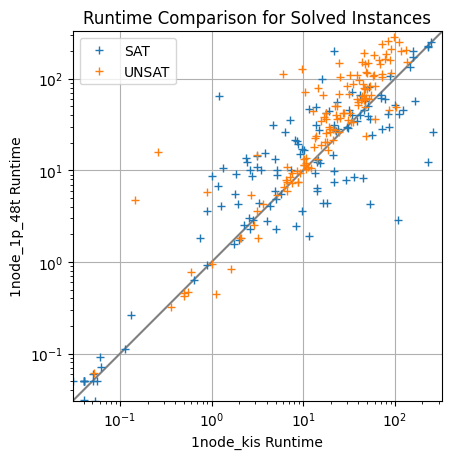
\includegraphics[scale=.5]{plots/square_runtime_compare/square_runtime_1node.png}
    \subcaption{1 node}
    \label{fig:runtimeCompare1node}
  \end{subfigure}
  \begin{subfigure}[c]{.4\textwidth}
    \center
    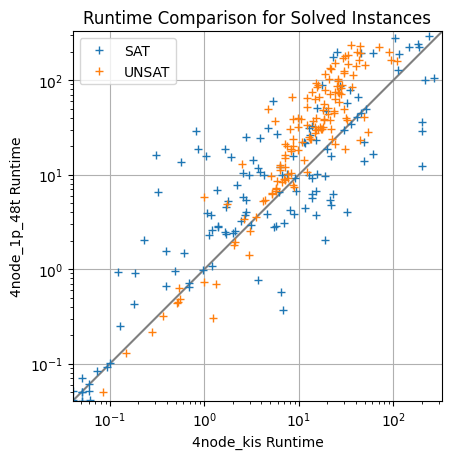
\includegraphics[scale=.5]{plots/square_runtime_compare/square_runtime_4node.png}
    \subcaption{4 node}
    \label{fig:runtimeCompare4node}
  \end{subfigure}
  \begin{subfigure}[c]{.4\textwidth}
    \center
    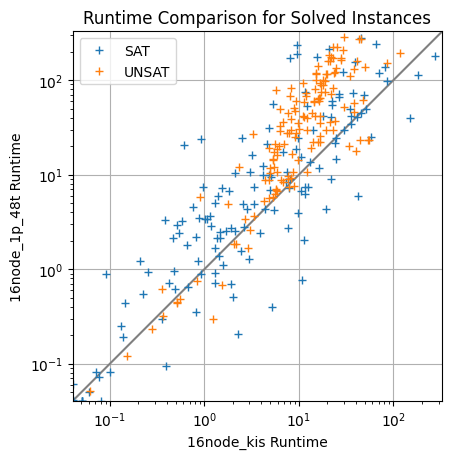
\includegraphics[scale=.5]{plots/square_runtime_compare/square_runtime_16node.png}
    \subcaption{16 node}
    \label{fig:runtimeCompare16node}
  \end{subfigure}
  \caption{Runtime Comparison between MallobSat and our algorithm}
  \label{fig:runtimeCompare}
\end{figure}

Figure \ref{fig:memCompare} shows the comparisons for the memory consumption between our approach and MallobSat in a similar manner, with MallobSat's peak memory consumption on the x-axis and the peak memory consumption of our algorithm on the y-axis. Again we differentiated into satisfiable and unsatisfiable instances. Here we can clearly see our approach consuming less memory in almost all cases.

\begin{figure}
  \center
  \begin{subfigure}[c]{.4\textwidth}
    \center
    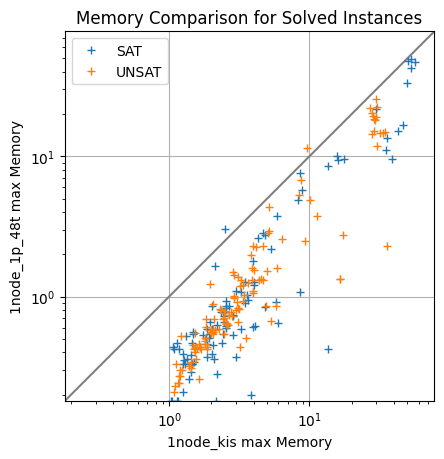
\includegraphics[scale=.5]{plots/square_mem_compare/square_mem_1node.png}
    \subcaption{1 node}
    \label{fig:memCompare1node}
  \end{subfigure}
  \begin{subfigure}[c]{.4\textwidth}
    \center
    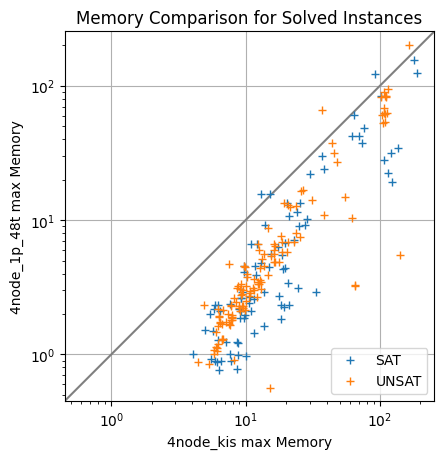
\includegraphics[scale=.5]{plots/square_mem_compare/square_mem_4node.png}
    \subcaption{4 node}
    \label{fig:memCompare4node}
  \end{subfigure}
  \begin{subfigure}[c]{.4\textwidth}
    \center
    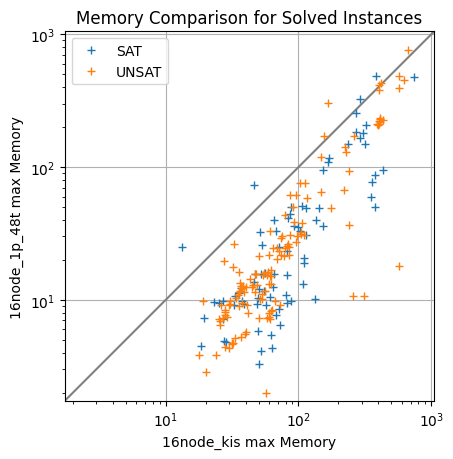
\includegraphics[scale=.5]{plots/square_mem_compare/square_mem_16node.png}
    \subcaption{16 node}
    \label{fig:memCompare16node}
  \end{subfigure}
  \caption{Memory Comparison between MallobSat and our algorithm}
  \label{fig:memCompare}
\end{figure}

The exact memory consumption of our algorithm as well as MallobSat is shown in figure \ref{fig:memAbsVars}. The mean memory Consuptions over all instances are shown in table \ref{tab:memMean}. For solved instances we find th ratio between MallobSat's mean memory consumption and the memory consumption of our algorithm to be $1.872$ for 1 node, $1.827$ for 4 nodes and $1.868$ for 16 nodes. For all instances we find the ratios to be a little smaller, with $1.897$ for 1 node, $1.66$ for 4 nodes and $1.725$ for 16 nodes.

\begin{figure}
  \center
  \begin{subfigure}[c]{.4\textwidth}
    \center
    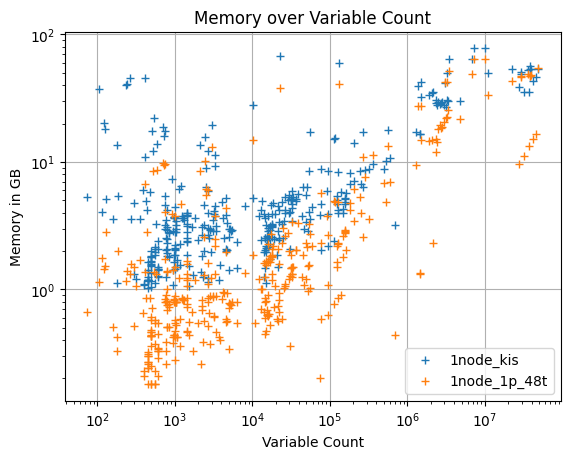
\includegraphics[scale=.3]{plots/1node_compare/mem_abs_over_vars.png}
    \caption{1 node}
  \end{subfigure}
  \begin{subfigure}[c]{.4\textwidth}
    \center
    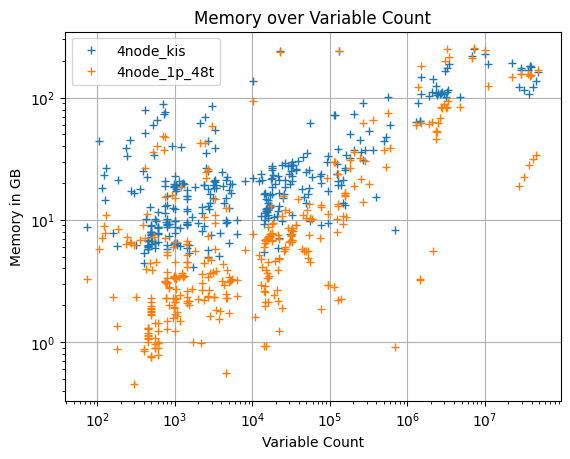
\includegraphics[scale=.3]{plots/4node_compare/mem_abs_over_vars.png}
    \caption{1 node}
  \end{subfigure}
  \begin{subfigure}[c]{.4\textwidth}
    \center
    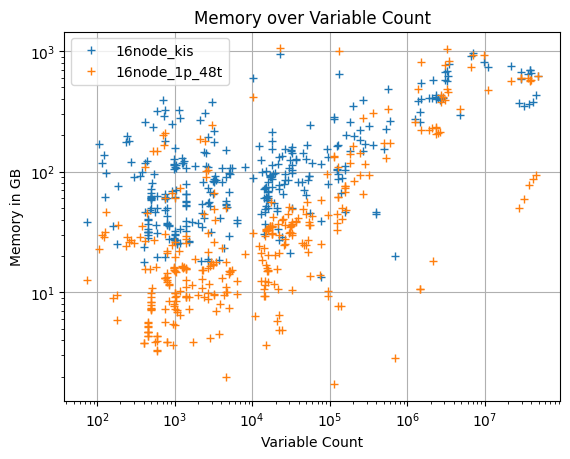
\includegraphics[scale=.3]{plots/16node_compare/mem_abs_over_vars.png}
    \caption{1 node}
  \end{subfigure}
  \caption{Memory consumption over variables.}
  \label{fig:memAbsVars}
\end{figure}

\begin{table}
  \center
  \begin{tabular}{ cccccc }
    \toprule
    \multicolumn{2}{c}{Setup} & \multicolumn{2}{c}{Solved Instances} & \multicolumn{2}{c}{All Instances}\\
    \#nodes & \#processors & Our Algorithm & MallobSat & Our Algorithm & MallobSat \\
    \midrule
    1  & 48  & 3.672GB & 6.875GB & 4.477GB & 8.494GB\\
    2  & 96  & 7.081GB & - & 9.321GB & -\\
    4  & 192 & 14.030GB & 25.631GB & 18.621GB & 30.921GB\\
    8  & 384 & 28.092GB & - & 37.700GB & -\\
    16 & 762 & 57.038GB & 106.534GB & 75.5967GB & 130.425GB\\
    \bottomrule
  \end{tabular}
  \caption{Mean memory consumption for number of processors}
  \label{tab:memMean}
\end{table}

\label{sec:peakMemRatios}
We now want to take a more detailed look into the memory consumption ratios. Figure \ref{fig:memRatiosVars} depicts the retio between the peak memory usage of MallobSat and our algorithm for all our benchmark instances. We distinguished between solved and un- or partially solved instances and depicted the 75-percentile for the speedups of all instances combined with a dashed line. The exact values of these 75-percentiles for all subplots are shown in table \ref{tab:memRatioPercentiles} The plots all mark the critical memory ratio of 1 with a drawn through black line.
% TODO: might not have been the right family for the name. Check families
In the top left corner of figure \ref{fig:memRatiosVars1node} we can see 6 instances with memory ratios over 29. The unsolved instances all belong to a family of instances called 'tseitin-formulas' encoding tseitin formulas. We want to use these instances as an example of an effect we observed on a few occations when comparing our algorithm to MallobSat: Our Algorithm seems to be more memory efficient on some unsolved instances. This phenomenon can be explained by the general pattern of SAT-solvers to accumulate memory usage over their runtime. Since Gimsatul already sacrifices runtime efficiency for shared memory clause sharing, our algorithm might simply not be as far into solving a specific instance at the timeout than MallobSat is. We therefore can not say that our algorithm is even more memory efficient in these scenarios, since by the time it solves the problem it will have accumulated more memory.
The same cluster contains a solved instance. It consists of only 180 variables and 432 clauses. Since it is satisfiable and does not appear as an outlier in figures \ref{fig:memRatiosVars4node} and \ref{fig:memRatiosVars16node} we assume our algorithm luckily found a satisfiable assignment unusually fast and consider this a true outlier.
% TODO? gibt 4 große Instanzen, für die gibts immer gute ratios:
% hwmcc17miters-xits-iso-oski15a08b08s.sanitized.cnf
% hwmcc17miters-xits-iso-oski15a08b00s.sanitized.cnf
% hwmcc17miters-xits-iso-6s281b35.sanitized.cnf
% hwmcc12miters-xits-iso-6s111.sanitized.cnf

TODO: more outlier discussion in plots

\begin{figure}
  \center
  \begin{subfigure}[c]{.4\textwidth}
    \center
    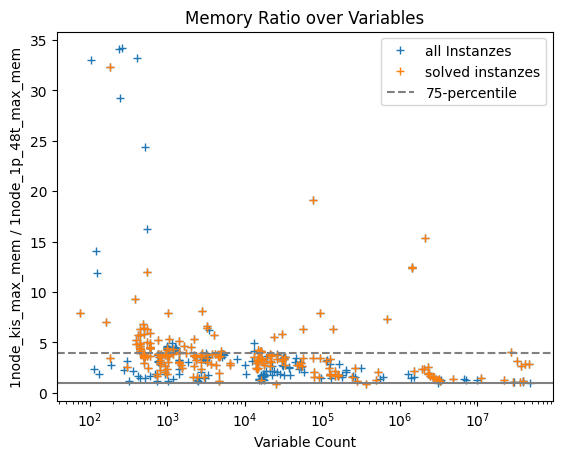
\includegraphics[scale=.3]{plots/1node_compare/mem_ratio_over_vars.png}
    \caption{1 node}
    \label{fig:memRatiosVars1node}
  \end{subfigure}
  \begin{subfigure}[c]{.4\textwidth}
    \center
    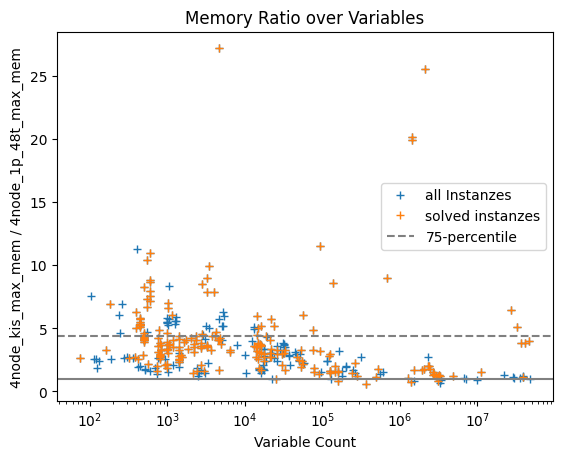
\includegraphics[scale=.3]{plots/4node_compare/mem_ratio_over_vars.png}
    \caption{4 node}
    \label{fig:memRatiosVars4node}
  \end{subfigure}
  \begin{subfigure}[c]{.4\textwidth}
    \center
    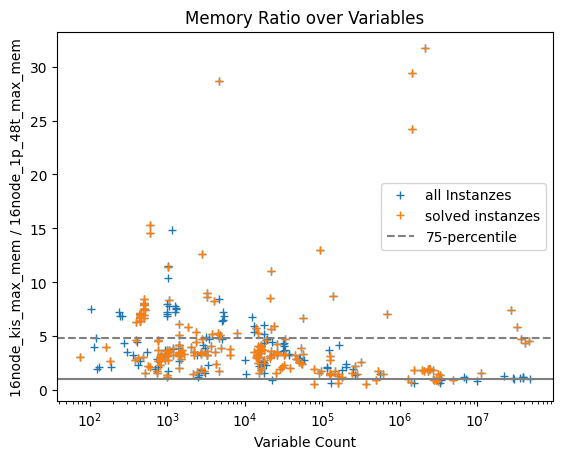
\includegraphics[scale=.3]{plots/16node_compare/mem_ratio_over_vars.png}
    \caption{16 node}
    \label{fig:memRatiosVars16node}
  \end{subfigure}
  \caption{Memory ratios over variables.}
  \label{fig:memRatiosVars}
\end{figure}

% 1node 75-percentile for all memory ratios: 3.9035953177257525
% 1node Geometric mean of geometric means: 0.2826566387020432

% 4node 75-percentile for all memory ratios: 4.376587301587302
% 4node Geometric mean of geometric means: 0.25621625192024783

% 16node 75-percentile for all memory ratios: 4.820217834212041
% 16node Geometric mean of geometric means: 0.21154183679147623

\begin{table}
  \center
  \begin{tabular}{ ccc }
    \toprule
    \#nodes & \#processors & 75-percentile \\
    \midrule
    1  & 48  & 3.904\\
    4  & 192 & 4.377\\
    16 & 762 & 4.820\\
    \bottomrule
  \end{tabular}
  \caption{Exact values of the 75-percentile for the ratios of peak memory consumption between MallobSat and our algorithm as described in section \ref{sec:peakMemRatios}}
  \label{tab:memRatioPercentiles}
\end{table}

\label{sec:GMs}
Up to this point we only ever discussed peak memory consumption. We now want to take a closer look at the relative memory consumption of our algorithm during the course of calculation. To give an overview we calculated the relative memory consumption of our algorithm to MallobSat for each second, that both solvers were active. E.g. if MallobSat finished its execution after 30s and our algorithm finished after 35s we calculated the ratio between MallobSat's memomry consumption and our algorithms memory consumption for every second of the first 30 seconds to compare their memory consumption during runtime only. Figure \ref{fig:memGmVars} shows the geometric means over these calculatedratios for each benchmark instance over the instance size by variable count. We marked the critical ratito of 1 with a dashed line and the geometric mean over all data points in a plot with a drawn through black line. The exact geometric means for each subplot are given in table \ref{tab:memGM}.

\begin{figure}
  \center
  \begin{subfigure}[c]{.4\textwidth}
    \center
    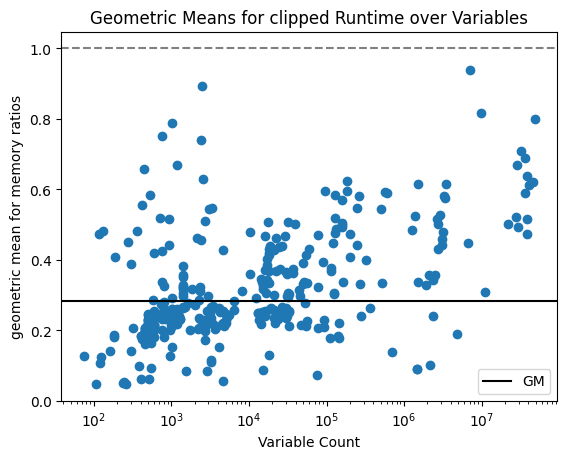
\includegraphics[scale=.3]{plots/1node_compare/mem_gm_over_vars.png}
    \caption{1 node}
  \end{subfigure}
  \begin{subfigure}[c]{.4\textwidth}
    \center
    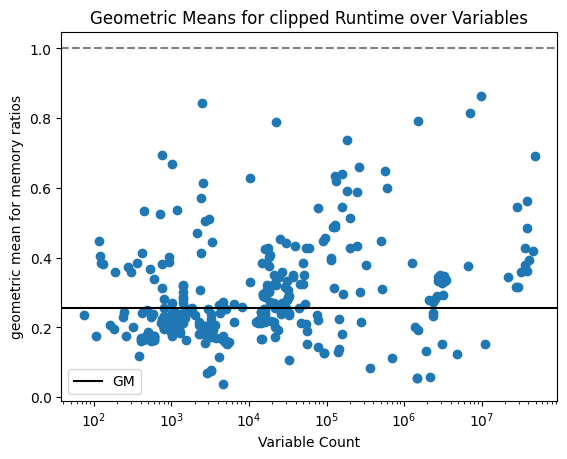
\includegraphics[scale=.3]{plots/4node_compare/mem_gm_over_vars.png}
    \caption{1 node}
  \end{subfigure}
  \begin{subfigure}[c]{.4\textwidth}
    \center
    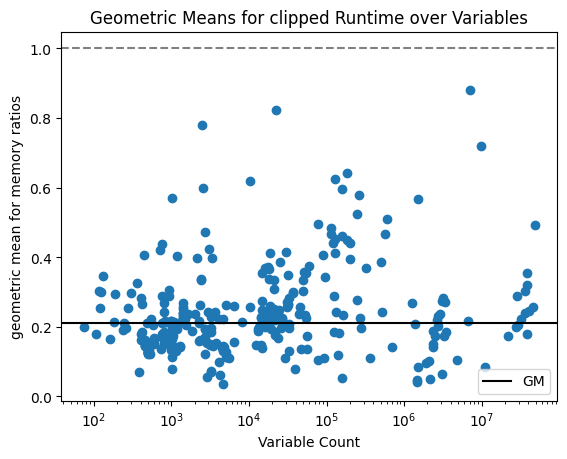
\includegraphics[scale=.3]{plots/16node_compare/mem_gm_over_vars.png}
    \caption{1 node}
  \end{subfigure}
  \caption{geometric means for memory ratios over variables.}
  \label{fig:memGmVars}
\end{figure}

\begin{table}
  \center
  \begin{tabular}{ ccc }
    \toprule
    \#nodes & \#processors & Geometric Mean \\
    \midrule
    1  & 48  & 0.283\\
    4  & 192 & 0.256\\
    16 & 762 & 0.212\\
    \bottomrule
  \end{tabular}
  \caption{Geometric Means of the geometric mean memory consumption per second as described in section \ref{sec:GMs}}
  \label{tab:memGM}
\end{table}

Figure \ref{fig:memRatiosSecs} shows the ratios between MallobSat and our algorithm per second for all benchmark instances that ran into our timeout of 300s. We smoothed the lines by plotting the geometric means over a sliding window of 5 seconds for each instance. 
The first obvious observation would be, that for almost all instances the lines stay below a ratio of 1, indicating a systematic reduction in memory consumption for our approach in comparison to MallobSat.
Our second interesting observation are the extreme jitters in some of our lines in the first few seconds of execution. We can explain these with a fairly simple effect of the search only setting of Mallob: At the start of the execution Mallob starts a preprocessing thread in addition to the regular solving threads. This thread solely executes the preprocessing techniques implemented in Kissat. After the preprocessing is finnished the solver threads already running on the unprocessed instance are slowly replaced by threads solving the preprocessed version of the problem formula. Since we get a memory status every second from Mallob we might get meassurements while a thread is beeing restarted a second offset for one of the two compared solvers, resulting in an extremely reduced memory consumption at this point in time and thus resulting in extreme jitters in our plots.

\begin{figure}
  \center
  \begin{subfigure}[c]{.4\textwidth}
    \center
    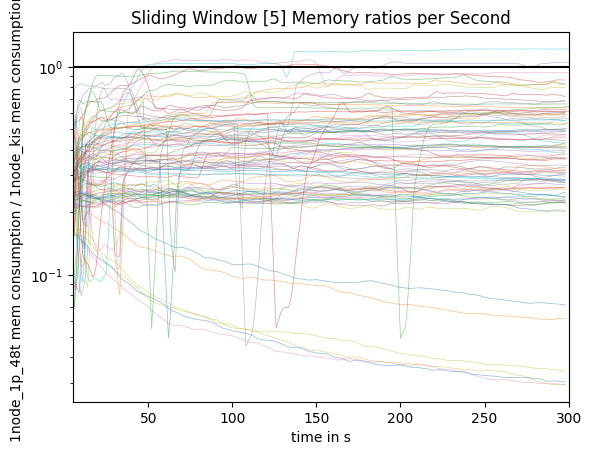
\includegraphics[scale=.3]{plots/1node_compare/mem_ratio_per_second.png}
    \caption{1 node}
  \end{subfigure}
  \begin{subfigure}[c]{.4\textwidth}
    \center
    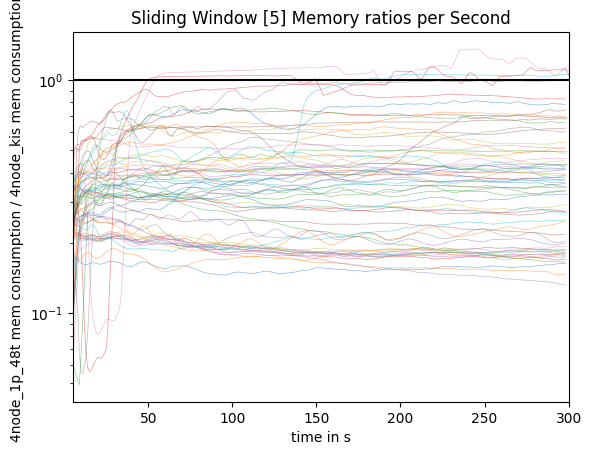
\includegraphics[scale=.3]{plots/4node_compare/mem_ratio_per_second.png}
    \caption{1 node}
  \end{subfigure}
  \begin{subfigure}[c]{.4\textwidth}
    \center
    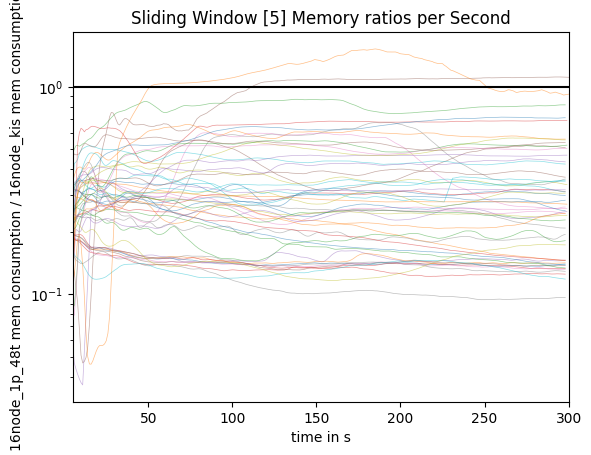
\includegraphics[scale=.3]{plots/16node_compare/mem_ratio_per_second.png}
    \caption{1 node}
  \end{subfigure}
  \caption{Memory ratios per second for all instances that ran the full 300s.}
  \label{fig:memRatiosSecs}
\end{figure}

% 1node 75-percentile for all memory ratios: 3.9035953177257525
% 1node Geometric mean of geometric means: 0.2826566387020432

% 4node 75-percentile for all memory ratios: 4.376587301587302
% 4node Geometric mean of geometric means: 0.25621625192024783

% 16node 75-percentile for all memory ratios: 4.820217834212041
% 16node Geometric mean of geometric means: 0.21154183679147623




\subsection{Miscallaneous Findings?}

TODO: Any interesting findings that have no other place. Collected Statistics for maybe?

%%%%%%%%%%%%%%%%%%%%%%%%%%%%%%%%%%%%%%%%%%%%%%%%%%%%%%%%%%%%%%%%%%%%%%

\newpage
\section{Conclusion}

\subsection{Runtime-Memory Tradeoff}

TODO: Is the longer runtime worth the saved memory?

\subsection{Usecases of our Algorithm}

TODO: In what situations would our algorithm be preferable to other approaches?

\subsection{Future Work}

TODO: write a (hopefully short) paragraph about what we didn't have time for anymore :(

%%%%%%%%%%%%%%%%%%%%%%%%%%%%%%%%%%%%%%%%%%%%%%%%%%%%%%%%%%%%%%%%%%%%%%

\clearpage

%%%%%%%%%%%%%%%%%%%%%%%%%%%%%%%%%%%%%%%%%%%%%%%%%%%%%%%%%%%%%%%%%%%%%%

\appendix

\section{Speedups per Family and Setup}
\label{app:speedupsFamiliesComplete}
\begin{longtable}{ lccccccc }
  \toprule
  family	&	\#	&	1node	&	2node	&	4node	&	8node	&	16node	&	gm speedup\\
  \midrule
  subset-cardinality	&	1	&	-	&	-	&	-	&	-	&	-	&	-\\
  hgen	&	1	&	-	&	-	&	59.623	&	130.885	&	1336.012	&	-\\
  binary-pigeon-hole	&	1	&	-	&	-	&	-	&	-	&	-	&	-\\
  binary-tree-parity	&	2	&	-	&	-	&	-	&	-	&	-	&	-\\
  coloring	&	8	&	-	&	-	&	-	&	-	&	-	&	-\\
  clique-width	&	1	&	-	&	-	&	-	&	-	&	-	&	-\\
  hamiltonian-cycle	&	1	&	-	&	-	&	7.99	&	8.607	&	9.199	&	-\\
  sgen	&	2	&	-	&	-	&	-	&	-	&	-	&	-\\
  risc-instruction-removal-subrv	&	2	&	-	&	-	&	-	&	-	&	-	&	-\\
  hypertree-decomposition	&	1	&	-	&	-	&	-	&	-	&	-	&	-\\
  fermat	&	1	&	-	&	-	&	-	&	-	&	-	&	-\\
  hardware-model-checking	&	1	&	-	&	-	&	-	&	-	&	-	&	-\\
  knights-problem	&	1	&	-	&	-	&	-	&	-	&	-	&	-\\
  waerden	&	1	&	-	&	-	&	-	&	-	&	-	&	-\\
  cril-misc	&	2	&	-	&	2.353	&	2.95	&	2.595	&	2.822	&	-\\
  relativized-pigeon-hole	&	2	&	-	&	-	&	-	&	-	&	-	&	-\\
  cryptography-simon	&	10	&	0.219	&	0.202	&	0.201	&	0.292	&	0.228	&	0.226\\
  heule-folkman	&	11	&	0.486	&	0.43	&	0.467	&	0.519	&	0.427	&	0.465\\
  subgraph-isomorphism	&	4	&	1.219	&	1.578	&	1.601	&	2.012	&	1.891	&	1.636\\
  puzzle	&	1	&	1.581	&	1.58	&	1.787	&	1.837	&	1.908	&	1.734\\
  miter	&	47	&	1.738	&	1.755	&	1.823	&	1.944	&	1.998	&	1.849\\
  st-connectivity-principle	&	2	&	2.651	&	2.027	&	2.504	&	2.74	&	2.68	&	2.506\\
  random-circuits	&	15	&	3.176	&	3.201	&	3.142	&	3.439	&	2.996	&	3.188\\
  automata-synchronization	&	1	&	2.694	&	3.297	&	3.425	&	3.326	&	3.4	&	3.216\\
  planning	&	6	&	2.573	&	3.069	&	2.182	&	4.431	&	4.779	&	3.254\\
  clique-formulas	&	1	&	3.452	&	3.743	&	3.75	&	3.54	&	3.767	&	3.648\\
  graph-isomorphism	&	1	&	3.292	&	3.727	&	3.558	&	3.642	&	4.085	&	3.652\\
  software-verification	&	15	&	2.253	&	3.525	&	4.873	&	4.831	&	4.355	&	3.821\\
  random-modularity	&	1	&	2.233	&	2.41	&	4.763	&	4.568	&	6.982	&	3.824\\
  cellular-automata	&	2	&	3.082	&	3.713	&	4.152	&	4.032	&	4.494	&	3.864\\
  bitvector	&	4	&	3.103	&	3.621	&	4.209	&	4.318	&	4.256	&	3.871\\
  stedman-triples	&	2	&	2.1	&	2.508	&	3.812	&	7.499	&	8.59	&	4.191\\
  erdos-discrepancy	&	1	&	2.216	&	5.008	&	4.424	&	6.39	&	7.165	&	4.681\\
  tseitin-formulas	&	8	&	4.768	&	4.857	&	5.087	&	5.356	&	5.416	&	5.09\\
  hardware-verification	&	5	&	4.608	&	5.503	&	5.616	&	5.816	&	5.726	&	5.435\\
  summle	&	3	&	2.857	&	6.792	&	4.843	&	6.344	&	8.389	&	5.493\\
  equivalence-chain-principle	&	4	&	4.899	&	5.982	&	6.331	&	6.466	&	7.245	&	6.135\\
  or\_randxor	&	1	&	5.818	&	5.787	&	7.144	&	7.039	&	7.28	&	6.579\\
  mutilated-chessboard	&	3	&	7.906	&	4.72	&	7.156	&	7.134	&	7.757	&	6.822\\
  scheduling	&	50	&	4.964	&	7.243	&	7.922	&	8.446	&	9.259	&	7.405\\
  rooks	&	3	&	7.324	&	8.081	&	9.091	&	6.64	&	7.402	&	7.664\\
  heule-nol	&	11	&	5.896	&	7.09	&	6.036	&	9.561	&	12.123	&	7.82\\
  quasigroup-completion	&	2	&	5.18	&	6.207	&	6.729	&	16.834	&	13.872	&	8.724\\
  grs-fp-comm	&	2	&	7.171	&	8.423	&	9.126	&	9.716	&	10.254	&	8.87\\
  cryptography-ascon	&	6	&	7.502	&	9.013	&	9.829	&	10.895	&	12.363	&	9.781\\
  popularity-similarity	&	1	&	10.449	&	10.079	&	9.65	&	10.861	&	10.935	&	10.383\\
  quantum-kochen-specker	&	10	&	9.283	&	10.743	&	10.469	&	10.917	&	10.954	&	10.454\\
  maxsat-optimum	&	13	&	7.797	&	11.306	&	11.407	&	13.962	&	15.845	&	11.734\\
  reg-n	&	4	&	0.545	&	27.772	&	28.21	&	26.609	&	27.9	&	12.595\\
  argumentation	&	21	&	12.448	&	16.472	&	17.132	&	19.12	&	20.399	&	16.879\\
  ramsey	&	1	&	12.11	&	19.653	&	17.338	&	18.754	&	19.133	&	17.143\\
  hamiltonian	&	40	&	9.402	&	15.061	&	18.36	&	21.842	&	30.853	&	17.73\\
  cryptography	&	7	&	6.98	&	15.289	&	19.646	&	26.816	&	31.87	&	17.81\\
  independent-set	&	15	&	17.084	&	19.857	&	21.196	&	23.342	&	24.077	&	20.956\\
  pythagorean-triples	&	1	&	9.899	&	20.955	&	19.668	&	23.807	&	55.926	&	22.233\\
  polynomial-multiplication	&	4	&	21.641	&	34.111	&	22.052	&	26.627	&	30.362	&	26.537\\
  minimum-disagreement-parity	&	17	&	32.697	&	31.982	&	29.057	&	37.168	&	49.981	&	35.508\\
  battleship	&	1	&	10.065	&	55.764	&	19.901	&	195.628	&	96.745	&	46.241\\
  unknown	&	1	&	24.193	&	53.217	&	40.007	&	71.647	&	70.288	&	48.172\\
  crafted-cec	&	1	&	22.625	&	21.583	&	128.892	&	29.699	&	197.845	&	51.713\\
  circuit-multiplier	&	1	&	51.034	&	25.529	&	68.564	&	78.517	&	62.533	&	53.507\\
  random-csp	&	2	&	19.592	&	76.009	&	32.096	&	93.696	&	106.327	&	54.394\\
  rbsat	&	5	&	49.344	&	43.944	&	57.652	&	191.928	&	126.86	&	78.828\\
  influence-maximization	&	1	&	42.347	&	200.995	&	49.984	&	164.3	&	164.761	&	102.865\\
  tree-decomposition	&	1	&	542.903	&	21.518	&	85.753	&	383.915	&	388.399	&	171.734\\
  \bottomrule
  \caption{Speedups per family and Solver Setup}
  \label{tab:speedupsFamiliesComplete}
\end{longtable}

\bibliographystyle{eptcs}
\bibliography{literatur}

\end{document}
